\chapter{Literature Review}\label{chap:literature}
\section{Introduction}
In this chapter, the research paper of different researchers around the world will be reviewed. The research on tuning the PWM controller signal, modification of phase current signal for minimizing the torque ripple as well as driving strategy for cars and trains will be reviewed.

\section{Torque Ripple}
Park, Sung Jun \textit{et al.} \citep{00824132} found that the back EMF generated by each of the three windings are slightly different in shape and magnitude from each other. Since the back EMF for each winding is different, therefore different phase current should be apply to each of the three windings. By assuming the three stator windings are in Y-shape connection, the cogging torque and the reluctance torque component is negligible and the mutual torque is directly proportional to the phase current, phase current for each of the three stator windings should be seperately excited in phase with the back EMF to minimize the losses and maximizing the torque-per-ampere generation.

Kim, Tae-Sung \textit{et al.} \citep{00976016} shows that by using the rectangular shape phase current that changes to high at the flat part of the back-emf wave can minimize the torque ripple, but this method is too ideal to be used in practical condition. In this paper, another method which is the unipolar PWM is introduced but it has a slow dynamic response, making this method not feasible at reducing the torque for current control commutation. The proposed current control algorithm is to seperate the phase current that contains all harmonic components to each harmonical components and then transformed into stationary frame. Then, each stationary frame is added together and the output is the current command. After this process, the rectangular wave will appear more rectangular and hence reducing the torque ripple.

Nam, Ki-Yong \textit{et al.} \citep{01608454} suggested reducing the torque ripple by varying the input voltage to the PMBLDC. The idea of this paper is that by maintaining the current at a constant value, the torque ripple could be minimized. The method for reducing the torque ripple used in this paper is to supply varied input voltage during the freewheeling region.

Wael A. Salah \textit{et al.} \citep{7648} proposed a method which apply a modified PWM signal to the PMBLDC. The modified PWM signal used will delay the build up of current in the in-coming phase gradually at low speed region. At high speed region, it will speed up the build up of current which results in overcoming the tips and dips of current during phase current commutation which contributes to reduce in torque ripple.

Mohamed. A. Enany \textit{et al.} \citep{285} presented a method for improving the performance of BLDC with varying the switch-on and switch-off angle of the phase current. By advancing the switch-on and switch-off phase current, it enables current at each windings to reach to the maximum value earlier hence reducing the tips and dips of the current at the other winding which results in reducing torque ripple.

G. H. Jang and C. J. Lee \citep{08305} proposed a method to reduce the torque ripple through eliminating cogging torque by implementing a modified current wave form. The modified current wave form consists of main and auxiliary wave which the main wave is the conventional wave whereas the auxiliary wave generates a torque which has the same magnitude but opposite direction to the cogging torque.

Vanisri A. and Devarajan N. \citep{1450216} describe the design of a controller with minimize torque ripple which different than the conventional controller for PMBLDC motor by filter components. The methodology of the method used in this research is passing through the signal through an inductor-capacitor filter which filters out the high frequency waveform. The capacitor is selected in a way that it can charge and discharge effectively and the inductor is responsible for reduce the current pulsation hence reducing the torque ripple.

Leila Parsa and Lei Hao \citep{04435197} studied the effect of magnetization, winding distribution, skew angle and current angle on torque pulsation minimization. The switching instance has been calculated in a way that the reluctance torque is utilized in reducing the torque pulsation. It is also shown in the paper that by using the proper switching interval and applying suitable current waveform, the torque pulsation is reduced. 

\section{Driving Strategy}

Michiel Koot \textit{et al.} \citep{01433223} showed the work of analysing the engine, battery and alternator of an Hybrid Electric Vehicle (HEV). After the value of the parameters of an HEV is discretized, Dynamic Programming (DP) and Quadratic Programming (QP) techniques are used for the control strategy of the HEV.

Phil Howlett \textit{et al.} \citep{5095} discussed the making of an optimal strategy for a solar powered vehicle on a level road for participation in the World Solar Challenge. The draft strategy pointed out in the paper is:

\begin{itemize}
	\item{Accelerate using maximum available power.}
	\item{Hold speed at a lower critical speed, V, until mid-morning.}
	\item{Follow solar power up to an upper critical speed, W.}
	\item{Hold speed W until mid-afternoon.}
	\item{Follow solar power back down to the lower critical speed, V.}
	\item{Hold speed V until late in the afternoon.}
	\item{Follow solar power.}
	\item{Apply full regenerative braking, if available, or coast.}
	\item{Apply full regenerative braking and mechanical braking.}
\end{itemize}

The mathematical model for the vehicle is built from the power flow from the solar panel to the traction system, from the battery to the traction system, from the solar panel to the battery and from the traction system to the battery. Vehicle dynamics, for instance, the rolling resistance and drag force were also modelled. Finally, the control strategy is made based on the mathematical model.

The paper written by Yasuo Shimizu \textit{et al.} \citep{03894304} introduced 2 system which is the Supervision Support System as shown in figure \ref{im:honda_supervision} and the Cruising Simulation as shown in figure \ref{im:honda_flowchart}. The Supervision Support System is a system where a control centre vehicle is followed behind the solar vehicle and collect all the data from the solar vehicle, the data is logged and calculated and the instruction is sent via transmitter back to the solar vehicle and displayed on the panel meters

\begin{figure}[htb]
	\centering
	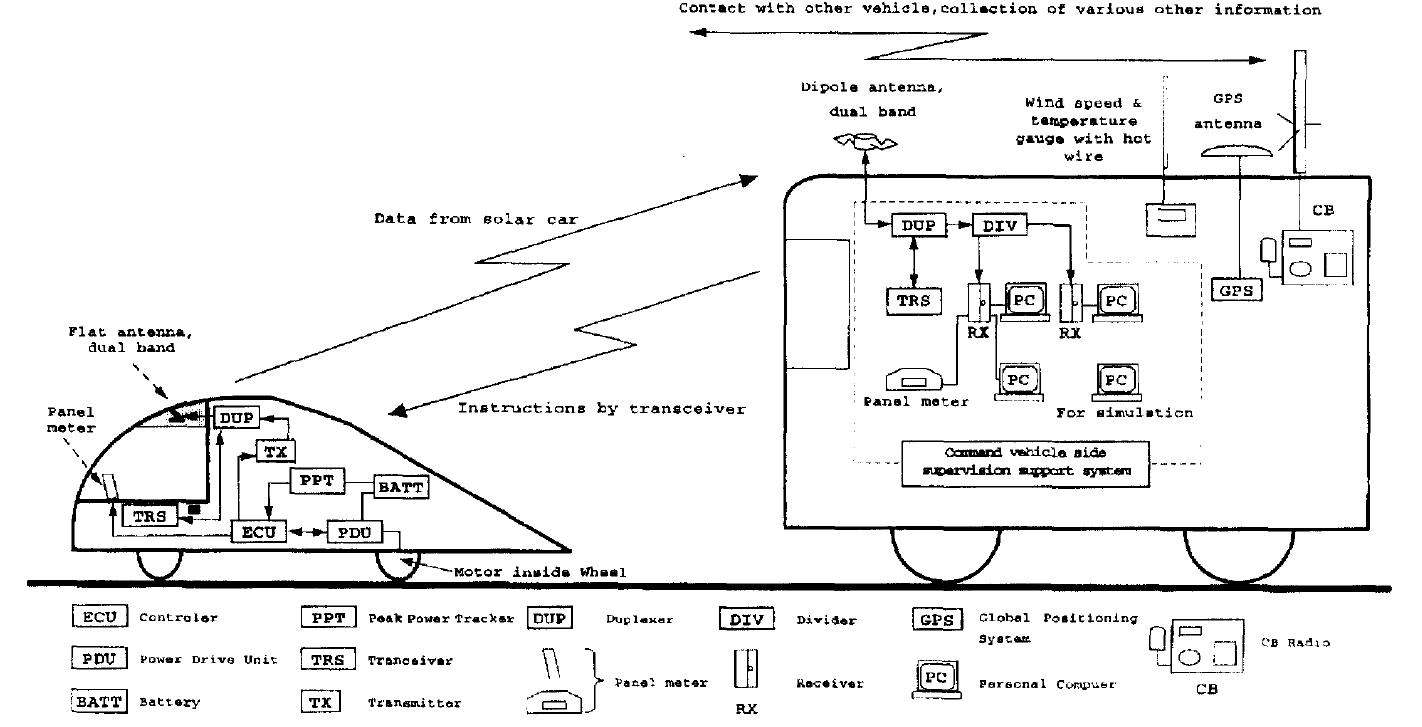
\includegraphics[width=6in]{images/honda_supervision.jpg}
	\caption{Supervision Support System hardware configuration schematic \citep{03894304}}
	\label{im:honda_supervision}
\end{figure}

The Cruising Simulation on the other hand is a simulation proccess where the condition component is set, for example, the environment condition settings, the vehicle specification settings and etc. Next, the result is calculated through calculation of every single condition, for instance, the reading of geographical data, the calculation of motor power and etc. By utilising the Supervision Support System and the Cruising Simulation, the on-road calculation could be done so that the power or speed control strategy can be set and implemented when the solar vehicle is running.

\begin{figure}[htb]
	\centering
	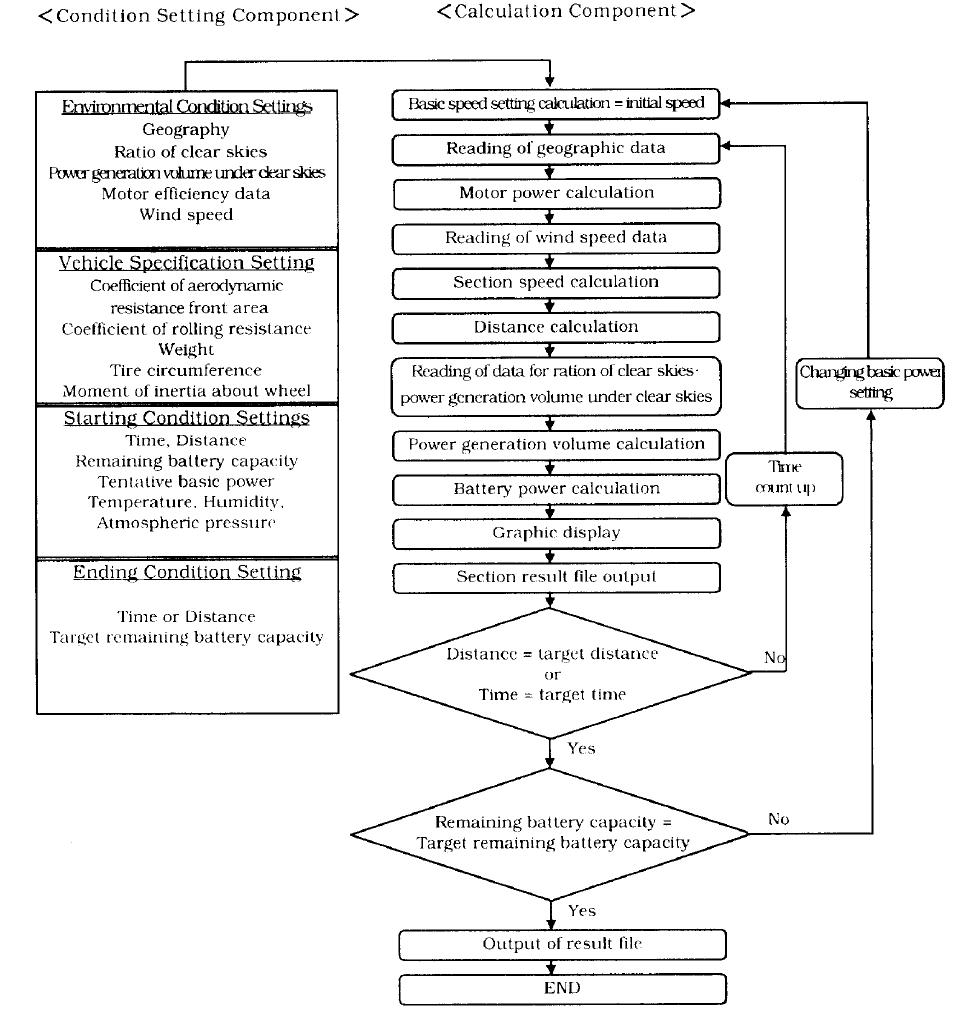
\includegraphics[width=5.5in]{images/honda_flowchart.jpg}
	\caption{Flowchart of the Cruising Simulation \citep{03894304}}
	\label{im:honda_flowchart}
\end{figure}\clearpage

Y.V. Bocharnikov \textit{et al.} \citep{04295937} researched on the optimal driving strategy for suburban railways. The strategy is constrained by two conditions which are energy saving and running fast so that it would not misses the schedule. There are 3 components for suburban railways which are the Motoring(M), Coasting(C) and Braking(B). By building mathematical model based on this 3 components and using fuzzy logic for optimization of energy function, a strategy with balance between the energy saving and running fast is achieved.

Peter Pudney and Phil Howlett \cite{s03342} described building of strategies for a train journey which have speed limits at certain part of the journey. The method used in this paper is to build mathematical model for both the vehicle model and the journey model. Then, the speed profile was build and the optimal driving strategies was derived using mathematical models.

\section{Summary}
